%%________________________________________________________________________
%% LEIM | PROJETO
%% 2022 / 2013 / 2012
%% Modelo para relatório
%% v04: alteração ADEETC para DEETC; outros ajustes
%% v03: correção de gralhas
%% v02: inclui anexo sobre utilização sistema controlo de versões
%% v01: original
%% PTS / MAR.2022 / MAI.2013 / 23.MAI.2012 (construído)
%%________________________________________________________________________
%%
%%
%% É importante ver o essencial do LaTeX antes de usar este template.
%% um bom "ponto de partida": http://en.wikibooks.org/wiki/LaTeX/
%%
%%________________________________________________________________________
%% Para alterar o Título, Nome dos Autores e Nome dos Orientadores fazer:
%% - abrir o ficheiro "00_PRJ_padrao.sty"
%% - procurar "Nome do aluno" e alterar
%% - procurar "número" e alterar; deixar os parêntesis
%% - procurar "Nome do orientador" e alterar
%% - procurar "[Doutor]" e atirar os parêntesis rectos ou eliminar tudo
%%
%% Caso precise de adicionar um novo aluno, ou orientador, deve:
%% - selecionar toda a linha (com "Nome do aluno" ou "Nome do orientador")
%% - seleccionar a linha imediatamente acima dessa
%% - copiar ambas as linhas
%% - colocar as linhas copiadas logo abaixo da primeira linha seleccionada
%%________________________________________________________________________





%% o documento é definido do tipo "book" em a4, font 12pt
\documentclass[a4paper,12pt,openany]{book}


%% para usar caracteres acentuados
%\usepackage[utf8]{inputenc} % no Unix (com codificação UTF-8)
\usepackage[utf8]{inputenc} % no Unix (com codificação UTF-8)

% para aspectos de hifenização (do Português)
\usepackage[portuguese]{babel}

%% para incluir imagens e tratar de modo adequado endereços url
\usepackage{graphicx,url}

%% para usar \begin{comment} ... \end{comment}
\usepackage{verbatim}

%% para usar o símbolo do euro
%usepackage{eurosym}

%% para juntar multiplas linhas em tabelas
\usepackage{multirow}

%% para usar símbolos matemáticos
\usepackage[centertags]{amsmath}

%% para usar \mathds{...}
\usepackage{dsfont}

%% para formatação (e.g. espaçamento) de Tabelas
\usepackage{tabls}

%% para usar listagens de código
\usepackage{listings}

%% para escrita "formal" de algoritmos
\usepackage{algorithm}

%% Para que a numeracao de listings seja global
%% (e nao no contexto de cada capitulo!)
\usepackage{chngcntr}

% para usar um estilo diferente na identificação de "Capítulo"
%Sonny, Lenny(x), Glenn, Conny, Rejne, Bjarne
%\usepackage[Lenny]{fncychap}
% Para ter no "heading" o nome do capítulo e da secção
\usepackage{fancyhdr}

% para usar hiperligações (especialmente relevante para o índice)
\usepackage[hidelinks]{hyperref}
%\hypersetup{linktocpage}
%\hypersetup{
%    colorlinks,
%    citecolor=black,
%    filecolor=black,
%    linkcolor=black,
%    urlcolor=black
%}

\usepackage{tcolorbox}
\tcbuselibrary{skins, breakable}

\newtcolorbox{promptbox}[1][]{
    breakable,
    enhanced,               % permite mais controlo
    frame empty,            % sem moldura padrão
    borderline west={0.4pt}{0pt}{black},
    borderline east={0.4pt}{0pt}{black},
    borderline north={0.4pt}{0pt}{black},
    borderline south={0.4pt}{0pt}{black},
    left=5mm,
    right=5mm,
    top=3mm,
    bottom=8mm,
    after skip=5mm,
    segmentation hidden,    % esconde linhas de segmentação entre quebras
    % Label só no final
    overlay last={%
        \node[anchor=east, inner sep=0pt, outer sep=0pt, yshift=-5mm] 
        at (frame.south east) {\small\textcolor{gray}{#1}};
    }
}


\usepackage[utf8]{inputenc}
\usepackage[T1]{fontenc}
\usepackage[portuguese]{babel}
\usepackage{booktabs}
\usepackage{array}
\usepackage{longtable}
\usepackage{xcolor}
\usepackage{colortbl}
\usepackage{ragged2e}
\usepackage{multirow}
 
\definecolor{headerblue}{RGB}{30,80,140}
\definecolor{lightgray}{RGB}{245,245,245}
\definecolor{simcolor}{RGB}{200,230,200}
\definecolor{naocolor}{RGB}{240,200,200}
\definecolor{parcialcolor}{RGB}{255,235,180}
 
\newcolumntype{P}[1]{>{\RaggedRight\arraybackslash}p{#1}}
%%________________________________________________________________________
%% para incluir o estilo proposto
\usepackage{./00_PRJ_padrao}
%%________________________________________________________________________



%%________________________________________________________________________
% mudar alguns nomes fixos para Português
%%________________________________________________________________________
% renomear "Listing" para "Código"
\renewcommand{\lstlistingname}{Código}
\addto\captionsportuges{
    \renewcommand{\contentsname}{Índice}}
\addto\captionsportuges{
    \renewcommand{\bibname}{Bibliografia}}
\addto\captionsportuges{
    \renewcommand{\proofname}{Prova}}
\addto\captionsportuges{
    \renewcommand{\chaptername}{Capítulo}}
\setlength{\headheight}{15pt}
%%________________________________________________________________________





%%________________________________________________________________________
%%%%%%%%%%%%%%%%%%%%%%%%%%%%%%%%%%%%%%%%%%%%%%%%%%%%%%%%%%%%%%%%%%%%%%%%%%
%% Begin Document
%%%%%%%%%%%%%%%%%%%%%%%%%%%%%%%%%%%%%%%%%%%%%%%%%%%%%%%%%%%%%%%%%%%%%%%%%%
\begin{document}
% para que a numeracao de listings seja global
% (e nao no contexto de cada capitulo!)
\counterwithout{lstlisting}{chapter}
%% incluir a capa
\frontmatter
\fazerCapa
%% incluir o resumo e abstract
%% caso pretenda, incluir os agradecimentos e a dedicatória
\frontmatter
%%________________________________________________________________________
%% comentar o que não interessar
%%%________________________________________________________________________
%% LEIM | PROJETO
%% 2022 / 2013 / 2012
%% Modelo para relatório
%% v04: alteração ADEETC para DEETC; outros ajustes
%% v03: correção de gralhas
%% v02: inclui anexo sobre utilização sistema controlo de versões
%% v01: original
%% PTS / MAR.2022 / MAI.2013 / 23.MAI.2012 (construído)
%%________________________________________________________________________




%%________________________________________________________________________
\myPrefaceChapter{Resumo}
%%________________________________________________________________________

O projeto Deep-Audio surge da necessidade de transcrição de áudios no trabalho da Polícia Judiciária, um processo demorado e cansativo quando feito manualmente. 

Desenvolvemos uma solução eficiente que facilitasse esta tarefa, utilizando modelos de inteligência artificial \textit{open-source}, como o Whisper da OpenAI, para converter áudio em texto, e o Pyannote, para identificar os oradores presentes no áudio. Além disso, o sistema permite corrigir possíveis falhas do modelo e gerar datasets para futuro treino de modelos.

As ideias mais relevantes incluem a criação de uma aplicação \textit{web} intuitiva, que transcreve áudios importados, permite a organização dos áudios em pastas, exibe as transcrições em formato de conversa (\textit{chat}) e permite edições quer do texto, quer do nome dos oradores por parte do utilizador.

O desenvolvimento do Deep-Audio seguiu uma abordagem iterativa e incremental, dividida em fases claras de forma a garantir uma melhor organização do fluxo de trabalho ao longo do tempo. 

Explorámos as tecnologias utilizadas para a transcrição e para a identificação de oradores, através da criação de protótipos para testar a integração entre as várias partes do sistema. Foram realizados testes incrementais em cada componente, desde o \textit{upload} de áudios até a exportação da transcrição final para um documento.

A interface gráfica foi desenvolvida com foco na usabilidade, incorporando \textit{feedback} dos utilizadores para ajustes nas funcionalidades e na própria interface. 

Esta abordagem metodológica permitiu um desenvolvimento estruturado, que possibilitou alcançar as metas pretendidas para o projeto.





%%________________________________________________________________________
\myPrefaceChapter{Abstract}
%%________________________________________________________________________

The Deep-Audio project arose from the need to transcribe audio in the work of the Judicial Police, a time-consuming and tiring process when done manually.

We developed an efficient solution that would make this task easier, using \textit{open-source} artificial intelligence models, such as Whisper from OpenAI, to convert audio into text, and Pyannote, to identify the speakers present in the audio. In addition, the system makes it possible to correct possible flaws in the model and generate datasets for future model training.

The most important ideas include the creation of an intuitive \textit{web} application, which transcribes imported audio, organizes the audio in folders, displays the transcripts in conversation format (\textit{chat}) and allows the user to edit both the text and the names of the speakers.

The development of Deep-Audio followed an iterative and incremental approach, divided into clear phases to ensure better organization of the workflow over time.

We explored the technologies used for transcription and speaker identification by creating prototypes to test the integration between the various parts of the system. Incremental tests were carried out on each component, from the \textit{upload} of audios to the export of the final transcript to a document.

The graphic interface was developed with a focus on usability, incorporating feedback from users to adjust the functionalities and the interface itself.

This methodological approach enabled structured development, which made it possible to achieve the project's goals.
%\include{./00b_PRJ_agradecimentos}
%%%________________________________________________________________________
%% LEIM | PROJETO
%% 2022 / 2013 / 2012
%% Modelo para relatório
%% v04: alteração ADEETC para DEETC; outros ajustes
%% v03: correção de gralhas
%% v02: inclui anexo sobre utilização sistema controlo de versões
%% v01: original
%% PTS / MAR.2022 / MAI.2013 / 23.MAI.2012 (construído)
%%________________________________________________________________________




%%________________________________________________________________________
\begin{myDedication}
%%________________________________________________________________________

Eventual texto de dedicatória \ldots

\vskip0.4in
\ldots mais texto,

\vskip0.8in
\ldots e o fim do texto.
    
    
\end{myDedication}
%%________________________________________________________________________





%% incluir a lista de conteúdos (índice, tabelas e figuras)
%comentar se quiser alterar o espaçamento entre linhas
\setlinespacing{1.15}
\myTableOfContents
%%________________________________________________________________________
%% comentar o que não interessar
%\myListOfTables
\myListOfFigures
%%________________________________________________________________________





%% "Corpo Principal" do texto
\mainmatter
\myPageStyle
%% cada um dos Capítulos
%% (aqui separados em dois ficheiros)
%%________________________________________________________________________
%% comentar o que não interessar (ou incluir outros ficheiros)
%%________________________________________________________________________
%% LEIM | PROJETO
%% 2022 / 2013 / 2012
%% Modelo para relatório
%% v04: alteração ADEETC para DEETC; outros ajustes
%% v03: correção de gralhas
%% v02: inclui anexo sobre utilização sistema controlo de versões
%% v01: original
%% PTS / MAR.2022 / MAI.2013 / 23.MAI.2012 (construído)
%%________________________________________________________________________




%%________________________________________________________________________
\chapter{Introdução}
\label{ch:introducao}
%%________________________________________________________________________

Este trabalho teórico-prático tem como objetivo: na primeira parte, desenvolver um modelo ontológico a partir de conceitos teóricos definidos em documentos oficiais da DGS no contexto da pandemia.

Na segunda parte, procedeu-se à resolução do caderno de exercícios sobre Lógica de Descrição, consolidando os fundamentos teóricos que estão como foco principal na avaliação deste trabalho. Sendo que esta parte não é abordada neste relatório.

Todos os exercícios foram resolvido à mão primeiramente e podem ser visto no PDF que acompanha o relatório. Partes dessas resoluções foram recortadas para enriquecer o relatório.


%%________________________________________________________________________
\chapter{Análise \texttt{person\_c1}}
\label{ch:anpc1}
%%________________________________________________________________________
%d

Para analisar a classificação de \texttt{person\_c1}, foi-se à aba \textit{DL Query} e, com o \textit{reasoner} ligado, procurou-se por \texttt{Confirmed} como mostra a figura abaixo:

\begin{figure}[htbp]
	\centering
	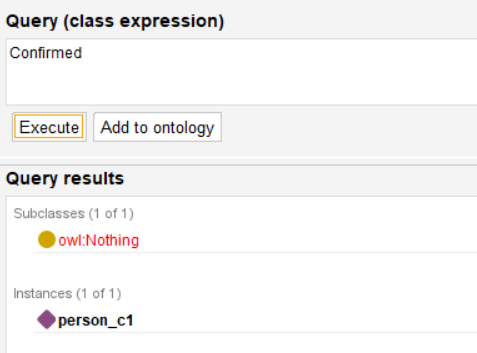
\includegraphics[width=0.7\textwidth]{an1.png}
	\caption{Consulta no Protégé para verificar a classificação de \texttt{person\_c1}}
	\label{fig:an1}
\end{figure}

Clicando na aba \textit{Classes} consultou-se a definição de \texttt{Confirmed} que era a seguinte:

\begin{center}
	\begin{verbatim}
		hasTestOutcomeOf some ({SARS-CoV-2-positive})
	\end{verbatim}
\end{center}

Para construir o \textit{tableau} consultou-se os slides do professor \cite[pág. 30]{Trigo_2025}.

Para verificar se uma instância é verdade, temos de negar esse conceito e verificar se existe \textit{clash}. Caso exista, o conceito é satisfeito.

Seguindo a ideia descrita acima fez-se a seguinte elaboração:

\[
\mathit{Confirmed} \equiv \exists\,\text{hasTestedOutcomeOf}.\text{SARS-CoV-2-positive}
\]

\[
\big(\mathcal{A} \models \text{Confirmed}(\text{person\_c1})\big)
\Leftrightarrow
\mathcal{A} \cup \{\neg\text{Confirmed}(\text{person\_c1})\}
\ \text{não-satisfeito em } \mathcal{T}
\]

\begin{figure}[htbp]
	\centering
	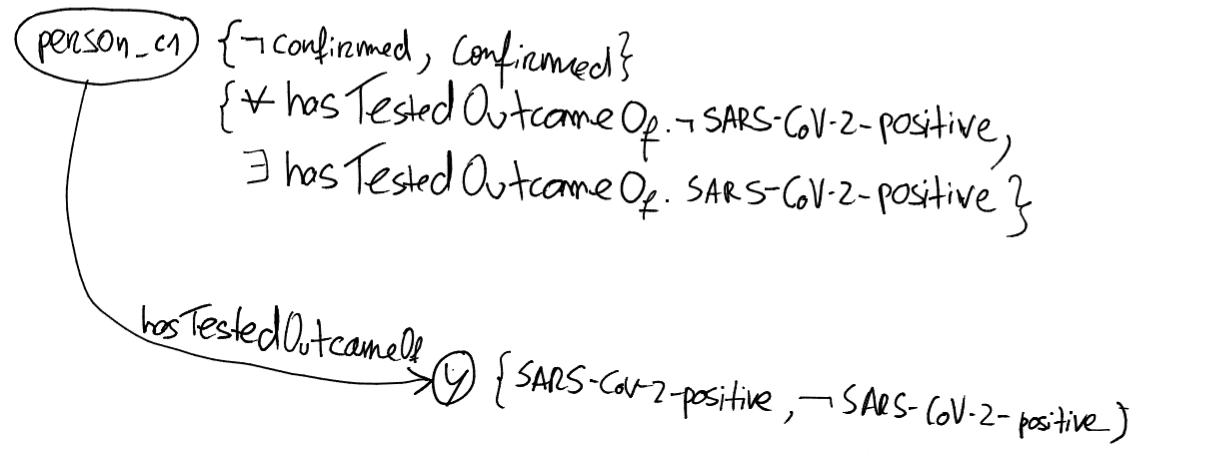
\includegraphics[width=0.7\textwidth]{an2.png}
	\caption{\textit{Tableau} para demonstrar classificação de \texttt{person\_c1}}
	\label{fig:an2}
\end{figure}

O Conceito é satisfeito, pois a negação de
$\text{Confirmed}(\text{person\_c1})$ não foi satisfeita, devido ao \textit{clash} presente na figura acima.
%%________________________________________________________________________
\chapter{Definir Relações}
\label{ch:defRel}
%%________________________________________________________________________

Neste ponto, tinha de se definir relações para que \texttt{person\_p2} fosse classificado como \textit{Probable}.

Ao consultar \texttt{person\_p2} no Protégé, verificou-se que este não tinha qualquer relação ou outro tipo de informação atribuída.

Desta forma, foi necessário fazer todas relações necessárias. E optou-se por adicionar \texttt{hasTestOutcomeOf SARS-CoV-2-not-conclusive} e \texttt{isExplainedBy \_none\_}. Isto, porque a definição de \textit{Probable} é: 

\begin{center}
	\begin{verbatim}
		((hasTestOutcomeOf value SARS-CoV-2-not-conclusive) or
		 (hasTestOutcomeOf value pan-coronavirus-positive))
		and (isExplainedBy value _none_)
	\end{verbatim}
\end{center}

Passando para uma expressão de Lógica de Descrição:

\begin{align*}
	\mathit{Probable} \equiv 
	& \Big(\exists\,\text{hasTestOutcomeOf}.\{\text{SARS-CoV-2-non-conclusive}\} \\
	& \quad \sqcup\ \exists\,\text{hasTestedOutcomeOf}.\{\text{pan-coronavirus-positive}\}\Big) \\
	& \quad \sqcap \exists\,\text{isExplainedBy}.\{\text{none}\}
\end{align*}

Também se demonstrou com a ajuda do \textit{tabelau} a classificação de \texttt{person\_p2}.

\begin{figure}[htbp]
	\centering
	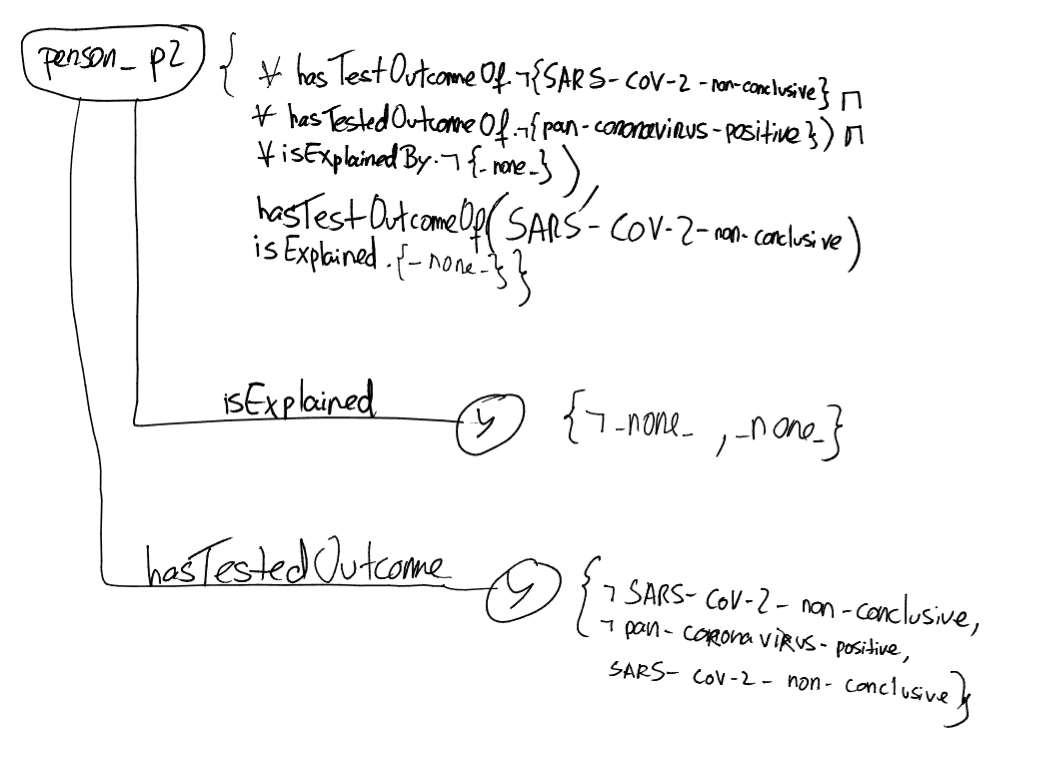
\includegraphics[width=0.7\textwidth]{an3.png}
	\caption{\textit{Tableau} para demonstrar classificação de \texttt{person\_p2}}
	\label{fig:an3}
\end{figure}

O conceito é satisfeito, pois a negação de
$\text{Probable}(\text{person\_p2})$ não foi satisfeita, devido ao \textit{clash} presente na figura acima.

Já no Protégé o resultado também foi satisfatório como demonstra a imagem recortada abaixo:

\begin{figure}[htbp]
	\centering
	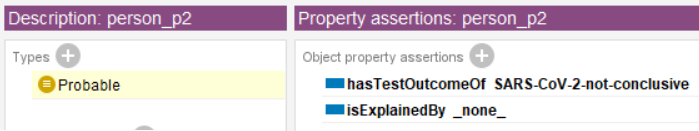
\includegraphics[scale=0.9]{an4.png}
	\caption{Resultados da classificação de \texttt{person\_p2} no Protégé}
	\label{fig:an4}
\end{figure}

%%________________________________________________________________________
\chapter{Definir conceito de \textit{Suspicious}}
\label{ch:sus}
%%________________________________________________________________________

Nesta alínea era preciso definir o conceito para o caso \textit{Suspicious}, tendo por base o documento oficial da DGS.

Realizou-se o seguinte raciocínio:

\textbf{Caso Suspeito}

\noindent $1$ - Infeção Respiratória (IR):
\[
\big(\text{IR} \sqcap (\text{VTA} \sqcup \text{RTA}) \sqcap E\{\text{none}\} \sqcap St\{14\}\big)
\]
(Viagem ($\text{VTA}$) ou Residência ($\text{RTA}$) com transmissão ativa, sem etiologia ($\text{E}$),
sintomas ($\text{St}$) c/14 dias)

\noindent $2$ - IR:
\[
\big(\text{IR} \sqcap (\text{CC}(\text{Cf} \sqcup \text{Prv}))\big) \sqcap St\{14\}
\]
(Contacto ($\text{CC}$) com caso confirmado ($\text{Cf}$) ou provável ($\text{Prv}$) de
SARS-CoV-2 ou COVID-19, sintomas c/14 dias)

\noindent $3$ - IR:
\[
\big(\text{IR} \sqcap M\{grh\} \sqcap E\{\text{none}\}\big)
\]
(Manifesta IR ($M$) grave, requer hospitalização ($\{grh\}$), sem etiologia)

\noindent obs: \textit{``grh''} é indivíduo de $\text{IR}$, \textit{logo} $M\{\text{IR}\}$.

Depois estas conclusões foram traduzidas para o Protégé da seguinte forma:

\begin{center}
	\begin{verbatim}
		(AcuteRespiratoryInfection
		and ((hasResidenceIn some AreaWithActiveCommunityTransmission) or 
		(hasTraveledFrom some AreaWithActiveCommunityTransmission))
		and (hasSymptomsStartingSince value _014-days-ago)
		and (isExplainedBy value _none_)) or
		(AcuteRespiratoryInfection
		and (hasContactWith some (Confirmed or Probable))
		and (hasSymptomsStartingSince value _014-days-ago)) or
		((hasManifestationOf some AcuteRespiratoryInfection)
		and (isExplainedBy value _none_))
	\end{verbatim}
\end{center}

%%________________________________________________________________________
\chapter{Verificações e trabalho no Protégé}
\label{ch:prot}
%%________________________________________________________________________

Na última parte do trabalho começou-se por verificar se \texttt{person\_s1} e \texttt{person\_s2} são corretamente classificadas como \textit{Suspicious}.

O \texttt{person\_s1} foi bem classificado logo de primeiro, mas o \texttt{person\_s2} teve de ter uma relação acrescentada: \texttt{isExplainedBy{\_none\_}}.

Desta forma, ambos os indivíduos ficaram bem classificados.

Depois, tinha-se de definir as relações necessárias para que \texttt{person\_s3} seja classificada como \texttt{Suspicious}. Como este indivíduo já tinha definido um tipo (\texttt{hasManifestationOf some AcuteRespiratoryInfection}), foi apenas preciso adicionar \texttt{isExplainedBy \_none\_}, tal qual na alínea anterior.

Por último, tinha-se de definir as relações necessárias para que \texttt{person\_s4} seja classificada como \texttt{Suspicious} e que estivesse em contacto com \texttt{person\_s2}.

Tal como no caso da \texttt{person\_s3}, foi necessário adicionar a relação \texttt{is ExplainedBy \_none\_} e, para representar a situação de contacto com \texttt{person \_s2}, também adicionou-se a relação \texttt{hasContactWith person\_s2}.
%%________________________________________________________________________
%% LEIM | PROJETO
%% 2022 / 2013 / 2012
%% Modelo para relatório
%% v04: alteração ADEETC para DEETC; outros ajustes
%% v03: correção de gralhas
%% v02: inclui anexo sobre utilização sistema controlo de versões
%% v01: original
%% PTS / MAR.2022 / MAI.2013 / 23.MAI.2012 (construído)
%%________________________________________________________________________


%%________________________________________________________________________
\chapter{Conclusão}
\label{ch:conclusão}
%%________________________________________________________________________

Este trabalho permitiu ganhar mais conhecimento sobre o funcionamento e a importância do \textit{tableau} para a verificação da satisfação dos conceitos e para verificar alguns dos exercícios realizados.

No restante, ganhou-se mais prática na analise com problemas deste tipo e a  imaginá-los como grafos, mas o grande aproveitamento deste trabalho incide principalmente sobre a componente teórica.
%%________________________________________________________________________




\appendix
%%________________________________________________________________________
%% comentar o que não interessar (ou incluir outros ficheiros)
%%%________________________________________________________________________
%% LEIM | PROJETO
%% 2022 / 2013 / 2012
%% Modelo para relatório
%% v04: alteração ADEETC para DEETC; outros ajustes
%% v03: correção de gralhas
%% v02: inclui anexo sobre utilização sistema controlo de versões
%% v01: original
%% PTS / MAR.2022 / MAI.2013 / 23.MAI.2012 (construído)
%%________________________________________________________________________




%%________________________________________________________________________
\chapter{Diagrama Sequencial}
\label{ch:diagramaSequencial}
%%________________________________________________________________________

\begin{figure}[h]
   \centering
   \includegraphics[width=18cm, angle=-90]{./seqDig}
   \caption{Diagrama Sequencial do fluxo das ações do projeto}
   \label{fig:uml2}
\end{figure}







%%________________________________________________________________________









%%________________________________________________________________________





%% bibliografia
%% estilo para construção de referências bibliográficas
%% PTS. Alterei o estilo "apalike" e chamei-lhe "apalikeMy".
%% Coloquei vários termos em Português
%% (e.g., "and", "of", "chapter", "editors", etc)
\nocite{*}
\bibliographystyle{apalikeMy}
\backmatter
\bibliography{XBib}


%%________________________________________________________________________
\end{document}
